\section{Results and Analysis}

\subsection{Quantitative Results}

As shown in Table~\ref{tab:experiment_results}, BiMBU consistently achieves the best performance across all crop sizes and input-channel configurations. For instance, at 256$\times$256 with VV+VH input, BiMBU reaches an MAE of 49.61, RMSE of 210.80, PSNR of 39.78\,dB, and SSIM of 0.9651, surpassing all baselines. At smaller crops, the gains are even more pronounced: with 64$\times$64 inputs, BiMBU improves SSIM to 0.9812 and PSNR to 44.14\,dB, while keeping MAE and RMSE lower than competing models. These results indicate that BiMBU preserves both pixel-level accuracy and structural similarity better than the baselines across all tested scales. Figure~\ref{fig:examples} shows 3 example visualizations of model outputs. From left to right: target Sentinel-2 image, BiMBU, GAN, SwinUnet, and UMamba.


\begin{table}
    \centering
    \renewcommand{\arraystretch}{1.2} % increase row height
    \caption{Quantitative results under different cropping sizes and input channel selections.}
    \label{tab:experiment_results}
    \begin{tabular}{lcccc}
    \hline
    \textbf{Model} & \textbf{MAE} $\downarrow$ & \textbf{RMSE} $\downarrow$ & \textbf{PSNR (dB)} $\uparrow$ & \textbf{SSIM} $\uparrow$ \\
    \hline
    
    % --- 256x256 ---
    \multicolumn{5}{c}{\textbf{Crop: 256$\times$256, Channels: VV+VH}} \\
    GAN      & 75.37 & 324.72 & 35.82 & 0.9338 \\
    SwinUnet & 60.09 & 253.32 & 37.97 & 0.9529 \\
    UMamba   & 67.03 & 288.88 & 36.65 & 0.9484 \\
    BiMBU    & \textbf{49.61} & \textbf{210.80} & \textbf{39.78} & \textbf{0.9651} \\
    \hline
    \multicolumn{5}{c}{\textbf{Crop: 256$\times$256, Channels: VV only}} \\
    GAN      & 79.32 & 337.56 & 35.66 & 0.9336 \\
    SwinUnet & 93.65 & 393.64 & 34.23 & 0.9281 \\
    UMamba   & 71.59 & 308.51 & 36.35 & 0.9466 \\
    BiMBU    & \textbf{59.99} & \textbf{247.50} & \textbf{38.26} & \textbf{0.9591} \\
    \hline
    \multicolumn{5}{c}{\textbf{Crop: 256$\times$256, Channels: VH only}} \\
    GAN      & 78.56 & 339.31 & 35.33 & 0.9328 \\
    SwinUnet & 82.72 & 348.25 & 35.05 & 0.9345 \\
    UMamba   & 76.55 & 328.45 & 35.60 & 0.9400 \\
    BiMBU    & \textbf{44.42} & \textbf{191.26} & \textbf{40.50} & \textbf{0.9673} \\
    \hline
    
    % --- 128x128 ---
    \multicolumn{5}{c}{\textbf{Crop: 128$\times$128, Channels: VV+VH}} \\
    GAN      & 69.57 & 295.12 & 37.12 & 0.9481 \\
    SwinUnet & 45.90 & 197.50 & 40.36 & 0.9652 \\
    UMamba   & 35.47 & 159.47 & 42.61 & 0.9749 \\
    BiMBU    & \textbf{31.05} & \textbf{137.48} & \textbf{43.85} & \textbf{0.9791} \\
    \hline
    \multicolumn{5}{c}{\textbf{Crop: 128$\times$128, Channels: VV only}} \\
    GAN      & 70.44 & 297.78 & 37.15 & 0.9481 \\
    SwinUnet & 90.35 & 379.52 & 34.60 & 0.9312 \\
    UMamba   & 44.37 & 198.13 & 40.82 & 0.9688 \\
    BiMBU    & \textbf{39.66} & \textbf{178.07} & \textbf{41.63} & \textbf{0.9720} \\
    \hline
    \multicolumn{5}{c}{\textbf{Crop: 128$\times$128, Channels: VH only}} \\
    GAN      & 70.24 & 298.88 & 37.23 & 0.9498 \\
    SwinUnet & 63.62 & 272.05 & 37.41 & 0.9498 \\
    UMamba   & 43.88 & 193.92 & 40.89 & 0.9684 \\
    BiMBU    & \textbf{33.96} & \textbf{151.92} & \textbf{42.96} & \textbf{0.9757} \\
    \hline
    
    % --- 64x64 ---
    \multicolumn{5}{c}{\textbf{Crop: 64$\times$64, Channels: VV+VH}} \\
    GAN      & 68.06 & 291.62 & 37.54 & 0.9545 \\
    SwinUnet & 41.58 & 181.62 & 41.11 & 0.9687 \\
    UMamba   & 35.14 & 158.47 & 42.67 & 0.9757 \\
    BiMBU    & \textbf{31.41} & \textbf{139.95} & \textbf{43.75} & \textbf{0.9797} \\
    \hline
    \multicolumn{5}{c}{\textbf{Crop: 64$\times$64, Channels: VV only}} \\
    GAN      & 70.48 & 300.88 & 37.10 & 0.9490 \\
    SwinUnet & 47.65 & 203.04 & 40.15 & 0.9648 \\
    UMamba   & 33.60 & 149.58 & 42.96 & 0.9749 \\
    BiMBU    & \textbf{30.09} & \textbf{134.05} & \textbf{44.14} & \textbf{0.9812} \\
    \hline
    \multicolumn{5}{c}{\textbf{Crop: 64$\times$64, Channels: VH only}} \\
    GAN      & 69.78 & 298.66 & 37.25 & 0.9491 \\
    SwinUnet & 45.00 & 194.12 & 40.54 & 0.9662 \\
    UMamba   & 38.83 & 175.52 & 41.92 & 0.9739 \\
    BiMBU    & \textbf{32.12} & \textbf{143.12} & \textbf{43.58} & \textbf{0.9787} \\
    \hline
    
    \end{tabular}
\end{table}


\begin{figure*}
    \centering
    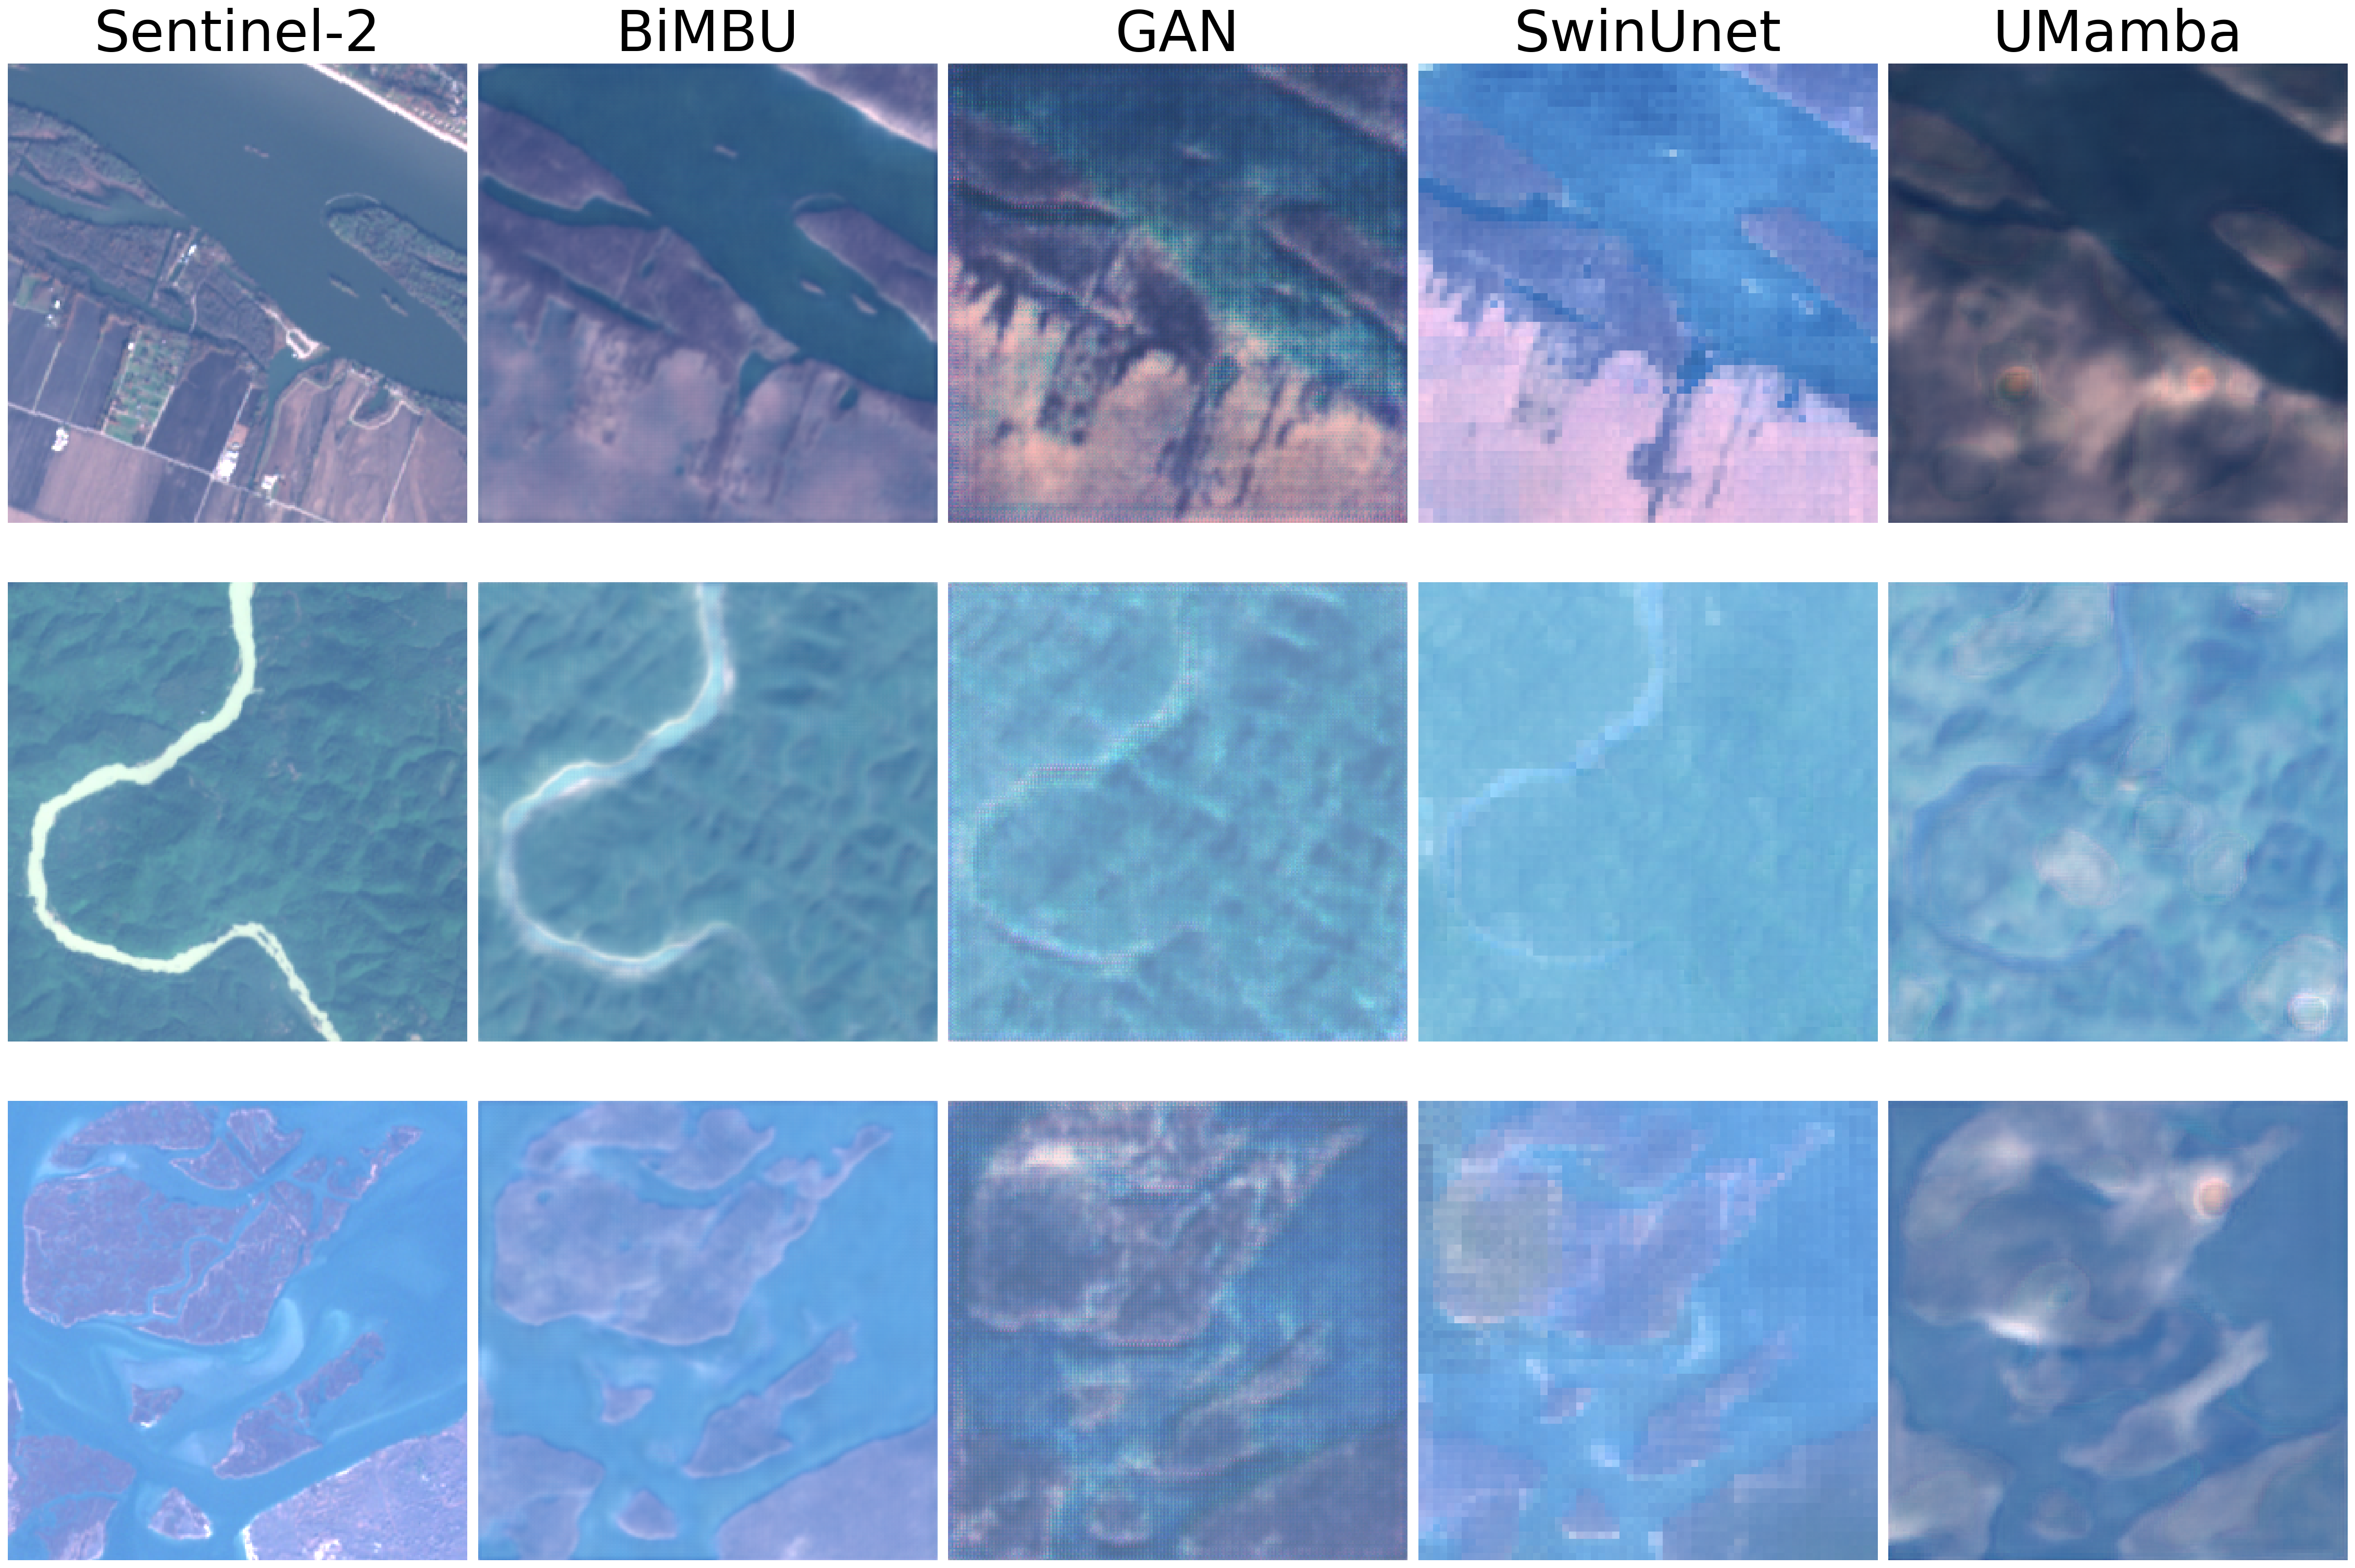
\includegraphics[width=.8\linewidth]{comparison-multi.png}
    \caption{Example visualizations of model outputs. From left to right: target Sentinel-2 image, BiMBU, GAN, SwinUnet, and UMamba.}
    \label{fig:examples}
\end{figure*}

\subsection{Spectral Shape and Index-based Evaluation}

Table~\ref{tab:spectral_index_eval} reports spectral-shape metrics and index-based errors. BiMBU obtains the lowest SAM (4.938) and SID (0.0169), showing closer agreement to the reference spectral signatures. For vegetation and water indices, BiMBU also yields the lowest errors: NDVI MAE of 0.0624 and RMSE of 0.0911, NDWI MAE of 0.0565 and RMSE of 0.0844, and NBR MAE of 0.0875 and RMSE of 0.1212. These values confirm that the reconstructed bands are suitable for downstream applications such as vegetation monitoring and water detection.


\begin{table*}
\centering
\renewcommand{\arraystretch}{1.2}
\caption{Spectral shape consistency (SAM, SID) and index-based evaluation (MAE and RMSE for NDVI, NDWI, and NBR) across models. $\downarrow$ indicates lower is better.}
\label{tab:spectral_index_eval}
\begin{tabular}{lcccccccc}
\hline
\textbf{Model} & \textbf{SAM} $\downarrow$ & \textbf{SID} $\downarrow$ & \textbf{NDVI MAE} $\downarrow$ & \textbf{NDVI RMSE} $\downarrow$ & \textbf{NDWI MAE} $\downarrow$ & \textbf{NDWI RMSE} $\downarrow$ & \textbf{NBR MAE} $\downarrow$ & \textbf{NBR RMSE} $\downarrow$ \\
\hline
GAN  & 8.274 & 0.0464 & 0.1090 & 0.1694 & 0.0971 & 0.1666 & 0.1147 & 0.1553 \\

SwinUnet & 6.048 & 0.0222 & 0.0731 & 0.1071 & 0.0652 & 0.1004 & 0.0961 & 0.1351 \\

UMamba   & 6.993 & 0.0297 & 0.0804 & 0.1134 & 0.0735 & 0.1074 & 0.1101 & 0.1534 \\


BiMBU   & \textbf{4.938} & \textbf{0.0169} & \textbf{0.0609} & \textbf{0.0911} & \textbf{0.0542} & \textbf{0.0844} & \textbf{0.0821} & \textbf{0.1212} \\

\hline
\end{tabular}
\end{table*}


\subsection{Per-Band Metrics}

Figure~\ref{fig:ssi-band} presents per-band SSIM values. BiMBU consistently outperforms the baselines across most Sentinel-2 bands. The largest margins appear in the near-infrared (B8) and shortwave infrared (B11, B12) bands, where BiMBU maintains SSIM above 0.96 while others fall below 0.95. These results highlight BiMBU’s ability to reconstruct bands with higher structural fidelity.

\begin{figure}
    \centering
    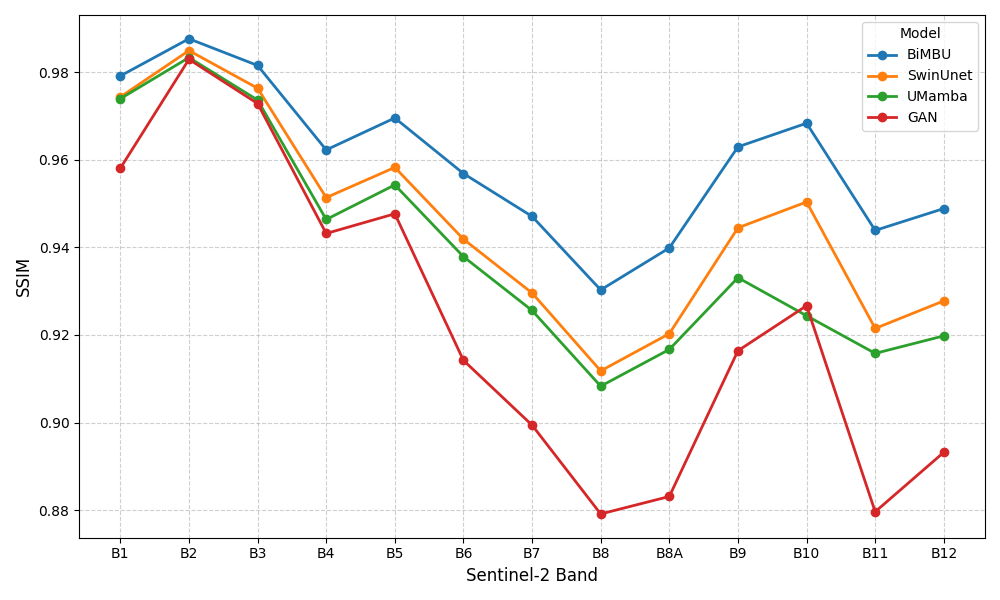
\includegraphics[width=\linewidth]{ssim_per_band.png}
    \caption{Per-band performance comparison of the BiMBU, SwinUnet, UMamba, and GAN models using the Structural Similarity Index (SSIM). The plot illustrates how the SSIM score for each model varies across the 13 different Sentinel-2 spectral bands.}
    \label{fig:ssi-band}
\end{figure}



\subsection{Computational Complexity}

Table~\ref{tab:model-complexity} summarizes model size and computational cost. BiMBU has 26.2M parameters and an inference time of 9.5\,ms, larger than UMamba (10.1M, 8.3\,ms) but smaller in multiply–accumulate operations (94.7\,G vs. 123.3\,G). Memory usage is higher (397.9\,MB), reflecting the model’s expanded capacity. These numbers show that BiMBU achieves accuracy improvements while maintaining tractable computational requirements.


\begin{table}
    \centering
    \caption{Model Complexity Analysis}
    \begin{tabular}{lccccc}
        \toprule
        \textbf{Model} & \makecell{\textbf{Params} \\ \textbf{(M)}} & \makecell{\textbf{Size} \\ \textbf{(MB)}} & \makecell{\textbf{Inference} \\ \textbf{(ms)}} & \makecell{\textbf{GPU Mem} \\ \textbf{(MB)}} & \makecell{\textbf{MACs} \\ \textbf{(G)}} \\
        \midrule
        GAN  & 54.43 & 217.73 & 2.10 & 346.16 & 19.48  \\
        SwinUnet & 27.15 & 108.61 & 8.93 & 177.44 & 7.78   \\
        UMamba   & 10.13 & 40.53  & 7.29 & 186.05 & 123.27 \\
        BiMBU   & 26.19 & 104.77 & 9.51 & 397.87 & 94.72  \\
        \bottomrule
        \label{tab:model-complexity}
    \end{tabular}
\end{table}



